\documentclass[12pt, a4paper]{article}
\usepackage{../notesheets}

%%%%%%%%%%%%%%%%%%%%%%%%%%%%%%%%%%%%%%%%%%%%%%%%%%
\author{Math 1220}
\title{Area and Volume Homework}
\date{}

\begin{document}
\maketitle
\nameline
%%%%%%%%%%%%%%%%%%%%%%%%%%%%%%%%%%%%%%%%%%%%%%%%%%
In this homework, we will compute some areas and volumes.
\begin{ex}
  Consider the function \(f(x) = \frac{1}{x}\). Find the area of the
  region bounded by \(y = f(x), y=0, x=-e^2,\) and \(x=-e\).
\end{ex}
\begin{ex}
  Let \(R\) be the region to the right of \(x=1\) bounded above by
  the curve \(y = f(x) = 
  \frac{1}{x}\) and bounded below by \(y=0\). Is the area of \(R\)
  finite or infinite? If
  it is finite, compute the area and if it is infinite, justify your answer.
\end{ex}
\pagebreak
\begin{ex}
  Now, take this region \(R\) and revolve it around the \(x\)-axis to
  create ``Gabriel's horn.'' Compute the volume of Gabriel's
  horn. (This picture, but solid instead of hollow.)\\
  
  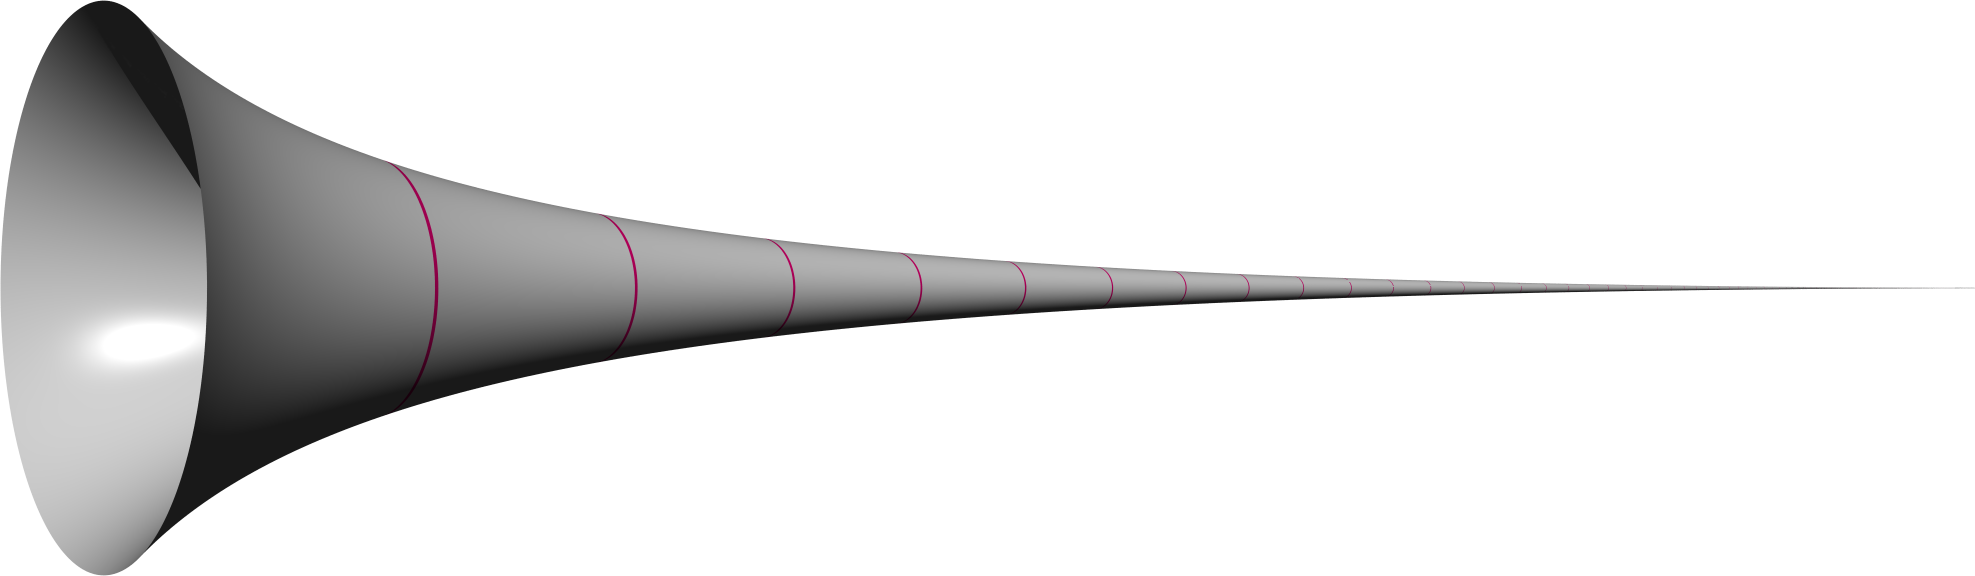
\includegraphics[scale=0.2]{images/GabrielHorn}
\end{ex}

%%%%%%%%%%%%%%%%%%%%%%%%%%%%%%%%%%%%%%%%%%%%%%%%%% 
\end{document}
